\begin{exercise}
Assume \(\cat{B}\) is a category with pullbacks.
Show that the functor \(\cat{B}^{\rightarrow\rightarrow} \to \cat{B}^\rightarrow\) sending \(\overset{f}{\to}\overset{g}{\to}\) to \(\overset{g}{\to}\) is a fibration.
Is the composite \(B^{\rightarrow\rightarrow} \to \cat{B}^{\rightarrow} \to \cat{B}\) also a fibration?
\end{exercise}

\begin{solution}
Let
\begin{align*}
\begin{tikzcd}[ampersand replacement=\&,]
\begin{pmatrix}
\begin{tikzpicture}
        \node(1){\(X\)}; 
        \node(2)[below of=1]{\(I\)};
        \draw[->](1)--node[right]{\scriptsize\(\varphi\)} (2);
\end{tikzpicture}
\end{pmatrix}
\arrow[r, "{(u, f)}"]
\&
\begin{pmatrix}
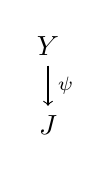
\begin{tikzpicture}
        \node(1){\(Y\)};
        \node(2)[below of=1]{\(J\)};
        \draw[->](1)--node[right]{\scriptsize\(\psi\)} (2);
\end{tikzpicture}
\end{pmatrix}
\end{tikzcd}
&&\text{i.e.,}
&&
\begin{tikzcd}[ampersand replacement=\&,]
X \arrow[r, "f"] \arrow[d, "\varphi"{left}] \& Y \arrow[d, "\psi"] \\
I \arrow[r, "u"] \& J
\end{tikzcd}
\end{align*}
be a morphism in \(\cat{B}^{\rightarrow}\), and let \(\begin{pmatrix}\begin{tikzcd}[row sep=small] B \arrow[d, "\beta"] \\ Y \arrow[d, "\psi"] \\ I\end{tikzcd}\end{pmatrix}\) be an object in \(\cat{B}^{\rightarrow\rightarrow}\) ``above'' \(\begin{pmatrix}\begin{tikzcd}[row sep=small] Y \arrow[d, "\psi"] \\ I\end{tikzcd}\end{pmatrix}\).
Since \(\cat{B}\) has pullbacks, let \(X \overset{\alpha}{\leftarrow} A \overset{q}{\rightarrow} B\) be a pullback of \(X \overset{f}{\to} Y \overset{\beta}{\leftarrow} B\). We claim that
\begin{align*}
\begin{tikzcd}[ampersand replacement=\&,]
\begin{pmatrix}
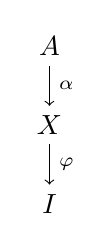
\begin{tikzpicture}
        \node(0){\(A\)};
        \node(1)[below of=0]{\(X\)}; 
        \node(2)[below of=1]{\(I\)};
        \draw[->](0)--node[right]{\scriptsize\(\alpha\)} (1);
        \draw[->](1)--node[right]{\scriptsize\(\varphi\)} (2);
\end{tikzpicture}
\end{pmatrix}
\arrow[r, "{(u, f, q)}"]
\&
\begin{pmatrix}
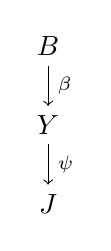
\begin{tikzpicture}
        \node(0){\(B\)};
        \node(1)[below of=0]{\(Y\)};
        \node(2)[below of=1]{\(J\)};
        \draw[->](0)--node[right]{\scriptsize\(\beta\)} (1);
        \draw[->](1)--node[right]{\scriptsize\(\psi\)} (2);
\end{tikzpicture}
\end{pmatrix}
\end{tikzcd}
&&\text{i.e.,}
&&
\begin{tikzcd}[ampersand replacement=\&,]
A \arrow[dr, phantom, " "{pullback}, very near start] \arrow[r, "q"] \arrow[d, "\alpha"{left}] \& B \arrow[d, "\beta"] \\
X \arrow[r, "f"] \arrow[d, "\varphi"{left}] \& Y \arrow[d, "\psi"] \\
I \arrow[r, "u"] \& J
\end{tikzcd}
\end{align*}
is a Cartesian lift of \((u, f)\).
Indeed, consider a situation as in the following diagram.
\begin{equation}
\label{eq:ex:1.1.9.diagram}
\begin{tikzcd}[row sep=small]
\begin{pmatrix}
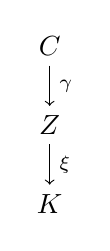
\begin{tikzpicture}
        \node(0){\(C\)};
        \node(1)[below of=0]{\(Z\)}; 
        \node(2)[below of=1]{\(K\)};
        \draw[->](0)--node[right]{\scriptsize\(\gamma\)} (1);
        \draw[->](1)--node[right]{\scriptsize\(\xi\)} (2);
\end{tikzpicture}
\end{pmatrix}
\arrow[dd, -Triangle]
\arrow[drr, bend left, "{(w, h, r)}"]
\arrow[dr, dashed, "?"]
\\[-10ex]
&
\begin{pmatrix}
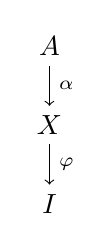
\begin{tikzpicture}
        \node(0){\(A\)};
        \node(1)[below of=0]{\(X\)}; 
        \node(2)[below of=1]{\(I\)};
        \draw[->](0)--node[right]{\scriptsize\(\alpha\)} (1);
        \draw[->](1)--node[right]{\scriptsize\(\varphi\)} (2);
\end{tikzpicture}
\end{pmatrix}
\arrow[r, "{(u, f, q)}"]
\arrow[dd, -Triangle]
&
\begin{pmatrix}
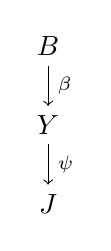
\begin{tikzpicture}
        \node(0){\(B\)};
        \node(1)[below of=0]{\(Y\)};
        \node(2)[below of=1]{\(J\)};
        \draw[->](0)--node[right]{\scriptsize\(\beta\)} (1);
        \draw[->](1)--node[right]{\scriptsize\(\psi\)} (2);
\end{tikzpicture}
\end{pmatrix}
\arrow[dd, -Triangle]
\\[-2ex]
\begin{pmatrix}
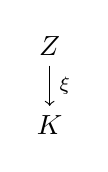
\begin{tikzpicture}
        \node(1){\(Z\)}; 
        \node(2)[below of=1]{\(K\)};
        \draw[->](1)--node[right]{\scriptsize\(\xi\)} (2);
\end{tikzpicture}
\end{pmatrix}
\arrow[dr, "{(v, g)}"{below left}]
\\[-2ex]
&
\begin{pmatrix}
\begin{tikzpicture}
        \node(1){\(X\)}; 
        \node(2)[below of=1]{\(I\)};
        \draw[->](1)--node[right]{\scriptsize\(\varphi\)} (2);
\end{tikzpicture}
\end{pmatrix}
\arrow[r, "{(u, f)}"]
&
\begin{pmatrix}
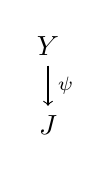
\begin{tikzpicture}
        \node(1){\(Y\)};
        \node(2)[below of=1]{\(J\)};
        \draw[->](1)--node[right]{\scriptsize\(\psi\)} (2);
\end{tikzpicture}
\end{pmatrix}
\end{tikzcd}
\end{equation}
(where necessarily \(w = u \circ v\) and \(h = f \circ g\)).
We must find a unique filler for the dashed morphism labeled ``\(?\)''; note that its first and second components are necessarily \(v\) and \(g\), respectively.
Also note that the diagram above is equivalent to the following one.
\begin{equation*}
\begin{tikzcd}
C \arrow[rr, bend left, "r"]  \arrow[d, "\gamma"] \arrow[r, dashed, "p"] & A \arrow[dr, phantom, " "{pullback}, very near start] \arrow[r, "q"] \arrow[d, "\alpha"] & B \arrow[d, "\beta"] \\
Z \arrow[r, "g"] \arrow[d, "\xi"] & X \arrow[r, "f"] \arrow[d, near end, "\varphi"] & Y \arrow[d, "\psi"] \\
K \arrow[r, "v"] \arrow[rr, bend right, "w"{below}] & I \arrow[r, "u"] & J
\arrow[from=ull, to=u, bend right, crossing over, near start, "h"{below}]
\end{tikzcd}
\end{equation*}
Here the dashed arrow \(p : C \to A\) is the unique morphism in \(\cat{B}\) such that \(g \circ \gamma = \alpha \circ p\) and \(r = q \circ p\), by virtue of \(X \overset{\alpha}{\leftarrow} A \overset{q}{\rightarrow} B\) being a pullback of \(X \overset{f}{\to} Y \overset{\beta}{\leftarrow} B\).
It follows that the unique filler for ``\(?\)'' in \eqref{eq:ex:1.1.9.diagram} is \(? = (v, g, p)\), so \((u, f, q)\) is a Cartesian lift of \((u, f)\), and hence the functor \(\cat{B}^{\rightarrow\rightarrow} \to \cat{B}^\rightarrow\) sending \(\overset{f}{\to}\overset{g}{\to}\) to \(\overset{g}{\to}\) is a fibration.

Moreover, the composite \(B^{\rightarrow\rightarrow} \to \cat{B}^{\rightarrow} \to \cat{B}\) is also a fibration since the composition of two fibrations is again a fibration (cf. \cite[Proposition~8.1.12]{MR1313497}, \cite[Proposition~3.7]{MR2222646}, \cite[Proposition~3.1]{MR0213413} \cite[Proposition~9.1.10]{MR4261588}) and since the codomain functor \(\cod : \cat{B}^{\rightarrow} \to \cat{B}\) is a fibration when \(\cat{B}\) has pullbacks (cf. \cite[Proposition~1.1.6]{MR1674451}).
\end{solution}